

\tikzset{every picture/.style={line width=0.75pt}} %set default line width to 0.75pt        

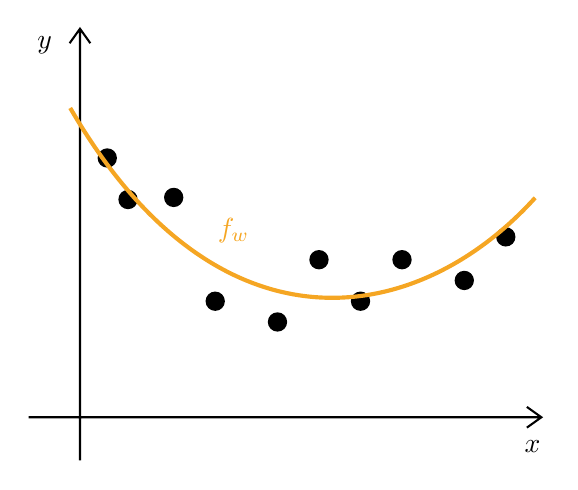
\begin{tikzpicture}[x=0.75pt,y=0.75pt,yscale=-1,xscale=1]
%uncomment if require: \path (0,300); %set diagram left start at 0, and has height of 300

%Shape: Axis 2D [id:dp6229280777631223] 
\draw  (34.29,224.06) -- (281.29,224.06)(58.99,36.86) -- (58.99,244.86) (274.29,219.06) -- (281.29,224.06) -- (274.29,229.06) (53.99,43.86) -- (58.99,36.86) -- (63.99,43.86)  ;
%Shape: Circle [id:dp061467044956021066] 
\draw  [fill={rgb, 255:red, 0; green, 0; blue, 0 }  ,fill opacity=1 ] (100,118.15) .. controls (100,115.86) and (101.86,114) .. (104.15,114) .. controls (106.44,114) and (108.29,115.86) .. (108.29,118.15) .. controls (108.29,120.44) and (106.44,122.29) .. (104.15,122.29) .. controls (101.86,122.29) and (100,120.44) .. (100,118.15) -- cycle ;
%Shape: Circle [id:dp46134600896432953] 
\draw  [fill={rgb, 255:red, 0; green, 0; blue, 0 }  ,fill opacity=1 ] (120,168.15) .. controls (120,165.86) and (121.86,164) .. (124.15,164) .. controls (126.44,164) and (128.29,165.86) .. (128.29,168.15) .. controls (128.29,170.44) and (126.44,172.29) .. (124.15,172.29) .. controls (121.86,172.29) and (120,170.44) .. (120,168.15) -- cycle ;
%Shape: Circle [id:dp6077179294298554] 
\draw  [fill={rgb, 255:red, 0; green, 0; blue, 0 }  ,fill opacity=1 ] (150,178.15) .. controls (150,175.86) and (151.86,174) .. (154.15,174) .. controls (156.44,174) and (158.29,175.86) .. (158.29,178.15) .. controls (158.29,180.44) and (156.44,182.29) .. (154.15,182.29) .. controls (151.86,182.29) and (150,180.44) .. (150,178.15) -- cycle ;
%Shape: Circle [id:dp362195154643858] 
\draw  [fill={rgb, 255:red, 0; green, 0; blue, 0 }  ,fill opacity=1 ] (170,148.15) .. controls (170,145.86) and (171.86,144) .. (174.15,144) .. controls (176.44,144) and (178.29,145.86) .. (178.29,148.15) .. controls (178.29,150.44) and (176.44,152.29) .. (174.15,152.29) .. controls (171.86,152.29) and (170,150.44) .. (170,148.15) -- cycle ;
%Shape: Circle [id:dp8081816475812211] 
\draw  [fill={rgb, 255:red, 0; green, 0; blue, 0 }  ,fill opacity=1 ] (190,168.15) .. controls (190,165.86) and (191.86,164) .. (194.15,164) .. controls (196.44,164) and (198.29,165.86) .. (198.29,168.15) .. controls (198.29,170.44) and (196.44,172.29) .. (194.15,172.29) .. controls (191.86,172.29) and (190,170.44) .. (190,168.15) -- cycle ;
%Shape: Circle [id:dp9676336222922068] 
\draw  [fill={rgb, 255:red, 0; green, 0; blue, 0 }  ,fill opacity=1 ] (210,148.15) .. controls (210,145.86) and (211.86,144) .. (214.15,144) .. controls (216.44,144) and (218.29,145.86) .. (218.29,148.15) .. controls (218.29,150.44) and (216.44,152.29) .. (214.15,152.29) .. controls (211.86,152.29) and (210,150.44) .. (210,148.15) -- cycle ;
%Shape: Circle [id:dp9372738784489105] 
\draw  [fill={rgb, 255:red, 0; green, 0; blue, 0 }  ,fill opacity=1 ] (240,158.15) .. controls (240,155.86) and (241.86,154) .. (244.15,154) .. controls (246.44,154) and (248.29,155.86) .. (248.29,158.15) .. controls (248.29,160.44) and (246.44,162.29) .. (244.15,162.29) .. controls (241.86,162.29) and (240,160.44) .. (240,158.15) -- cycle ;
%Shape: Circle [id:dp022406622313395186] 
\draw  [fill={rgb, 255:red, 0; green, 0; blue, 0 }  ,fill opacity=1 ] (260,137.15) .. controls (260,134.86) and (261.86,133) .. (264.15,133) .. controls (266.44,133) and (268.29,134.86) .. (268.29,137.15) .. controls (268.29,139.44) and (266.44,141.29) .. (264.15,141.29) .. controls (261.86,141.29) and (260,139.44) .. (260,137.15) -- cycle ;
%Shape: Circle [id:dp8149691081145218] 
\draw  [fill={rgb, 255:red, 0; green, 0; blue, 0 }  ,fill opacity=1 ] (68,99.15) .. controls (68,96.86) and (69.86,95) .. (72.15,95) .. controls (74.44,95) and (76.29,96.86) .. (76.29,99.15) .. controls (76.29,101.44) and (74.44,103.29) .. (72.15,103.29) .. controls (69.86,103.29) and (68,101.44) .. (68,99.15) -- cycle ;
%Shape: Circle [id:dp4028862229737822] 
\draw  [fill={rgb, 255:red, 0; green, 0; blue, 0 }  ,fill opacity=1 ] (78,119.15) .. controls (78,116.86) and (79.86,115) .. (82.15,115) .. controls (84.44,115) and (86.29,116.86) .. (86.29,119.15) .. controls (86.29,121.44) and (84.44,123.29) .. (82.15,123.29) .. controls (79.86,123.29) and (78,121.44) .. (78,119.15) -- cycle ;
%Curve Lines [id:da7352658004300567] 
\draw [color={rgb, 255:red, 245; green, 166; blue, 35 }  ,draw opacity=1 ][line width=1.5]    (54.29,75.05) .. controls (124.29,196.05) and (220.29,182.32) .. (278.29,118.32) ;



% Text Node
\draw (277,238) node   {$x$};
% Text Node
\draw (42,45) node   {$y$};

\draw (133,134) node [color={rgb, 255:red, 245; green, 166; blue, 35 }  ,opacity=1 ]  {$f_w$};

\end{tikzpicture}
